\chapter{Heuristic}
\label{ch:heuristic}

We present a fast approach to decide problem~\ref{prob:weak-udc-lobster} on a lobster instance of size $n$. Like the dynamic program from the previous chapter, it runs in time linear in $n$. The basic idea, to impose an order on the graph nodes and pick embedding coordinates step by step, remains the same. However it eliminates the large constant factor in the number of sub-problems considered.

This is a greedy algorithm: Instead of branching into different sub-problems, we immediately commit to a final placement decision at every step. This decision is based only on information that is obtainable in a short constant amount of time. Through this shortcut, we process only one sub-problem at each depth $0 \leq d \leq n$.

The price for the resultant speedup is correctness. In some cases, the heuristic decision prematurely commits us to embed a vertex at coordinates that are incompatible with any valid embedding, even if some valid embedding exists. The heuristic algorithm yields false negative answers in these cases.

\section{Algorithm Definition}

The heuristic algorithm decides problem~\ref{prob:weak-udc-lobster} on a lobster $G = (V, E)$ by incrementally constructing a series of partial embedding functions $d_0, \ldots, d_n \colon V \to \reals^2$.

We reuse some concepts from the dynamic programming approach as defined in Section~\ref{section:ch4-probdef}. Again, the algorithm assigns coordinates to vertices in a globally determined admissible embedding order $\order$. We also call this the \emph{depth-first} order, explicitly denoted as $\order^D$, to distinguish it from the variant in Section~\ref{section:ch5-bfs}. When we construct $d_{i+1}$ from $d_i$, we refer to the bipartition $V = V_d \dotcup V_r$. The prefix $V_d$ is the same as the domain of the partial embedding function $d_i$. We consider $V$ to be an ordered set, explicitly referred to as $V_{\order}$, and denote by $v_i$ the $i$-th vertex in the ordered set.

The algorithm starts from $d_0(v)$ defined on the empty domain, with no coordinates assignment to any $v$. It iteratively derives the successor function $d_{i+1}$ by considering $v_{i+1}$, the next vertex in order.
The partial function expands to include the embedding coordinates for $v_{i+1}$ determined by the heuristic function:

\begin{equation*}
    d_{i+1}(v) := \begin{cases} \texttt{heuristic}(v, d_i) & \text{if } v = v_{i+1},\\ d_i(v)& \text{otherwise}. \end{cases}
\end{equation*}

The result is ``yes'' if the algorithm completes the embedding function $d = d_n$, and ``no'' if the heuristic function fails to find valid coordinates for some $v_i$.

\section{Heuristic Function}

Given the vertex $v_{i+1}$ and partial embedding function $d_i$, the heuristic function selects the next embedding coordinates $$\kappa \in \Gamma(d_i(p(v_{i+1}))) \setminus \{ \coord \mid \exists v: d_i(v) = \coord \},$$ where $p(v_{i+1})$ is the parent vertex of $v_{i+1}$. In other words, $\kappa$ represents a disk adjacent to the disk of the parent vertex which does not overlap any previously selected coordinates. The heuristic function should attempt to pick the most promising of the at most 5 candidates in this set.

Our design goals for a heuristic which produces promising candidates are:

\begin{enumerate}
    \item\label{dg_bend} Spine disks should, within the constraints of x-monotonicity, be appended such that there is as much free space around them as possible. The relevant area around them extends up to two units of distance, where leaves may be assigned.
    \item\label{dg_back} Branch and leaf disks should not block vital coordinates for later vertices. Since we know that the spine will be x-monotone, going in some forward direction, it makes sense to embed the current vertex far back to keep it out of the way.
    \item\label{dg_balance} Bends in the spine might be unavoidable. Yet, by placing branches on both sides in a balanced way, the spine naturally flows in the in-between forward direction. This avoids conflicts with the x-monotonicity restriction.
    \item\label{dg_space} A branch should always have space to fit its leaves in the neighborhood. Knowing that fewer blocked coordinates and therefore more free space can be expected in the forward direction, we should avoid placing a branch so far back that the surrounding space will be obviously insufficient.
\end{enumerate}

Before we define criteria realizing these design goals, we need some supporting concepts.

Let $\coord$ be a tri-grid x-/y-coordinate. The set of \emph{two-step neighbors}

\begin{equation*}
\Gamma^2(\coord) = \bigcup\limits_{c \in \Gamma(\coord)} \Gamma(c) \setminus \{ \coord \}
\end{equation*}

is the set of all tri-grid coordinates at which another vertex $v$ of graph distance $\leq 2$ to $\coord$ could generally be placed. These are all vertices $v$ such that, for any lobster $G = (V, E)$, $(\coord, v) \in E$ or $\exists u: (\coord, u) \in E \wedge (u, v) \in E$.

Let $d_i$ be a partial embedding function which assigns coordinates to the first $i$ vertices in $V_{\order}$. We define the \emph{free space} $f(i, \cdot)$ as a function counting unassigned tri-grid coordinates in $d_i$. Free space may apply to a particular x-/y-coordinate $a$ or a set of coordinates $A$.

\begin{equation*}
\begin{aligned}
f(i, a) &= \begin{cases}1 & \text{ if } \nexists v_k \in V_{\order}: k \leq i \wedge d_i(v_k) = a \\ 0 & \text{ otherwise} \end{cases}\\
f(i, A) &= \sum\limits_{a \in A} f(i, a)
\end{aligned}
\end{equation*}

We represent a \emph{direction} by a unit vector at angle $\beta$ relative to the x-axis, denoted with $\overrightarrow e(\beta) = (\cos \beta, \sin \beta)$.

Let $d_i, i > 0$ be a partial embedding function and $\coord_s = d_i(v_j) = (x_s, y_s)$ be the coordinates of the maximum embedded spine vertex $v_j$, with index $j \leq i$. Then $\alpha \in \{ \overrightarrow e(-60^\circ), \overrightarrow e(0^\circ), \overrightarrow e(60^\circ) \}$ is the \emph{principal direction} in which we want to extend the spine.

\begin{figure}
    \centering
    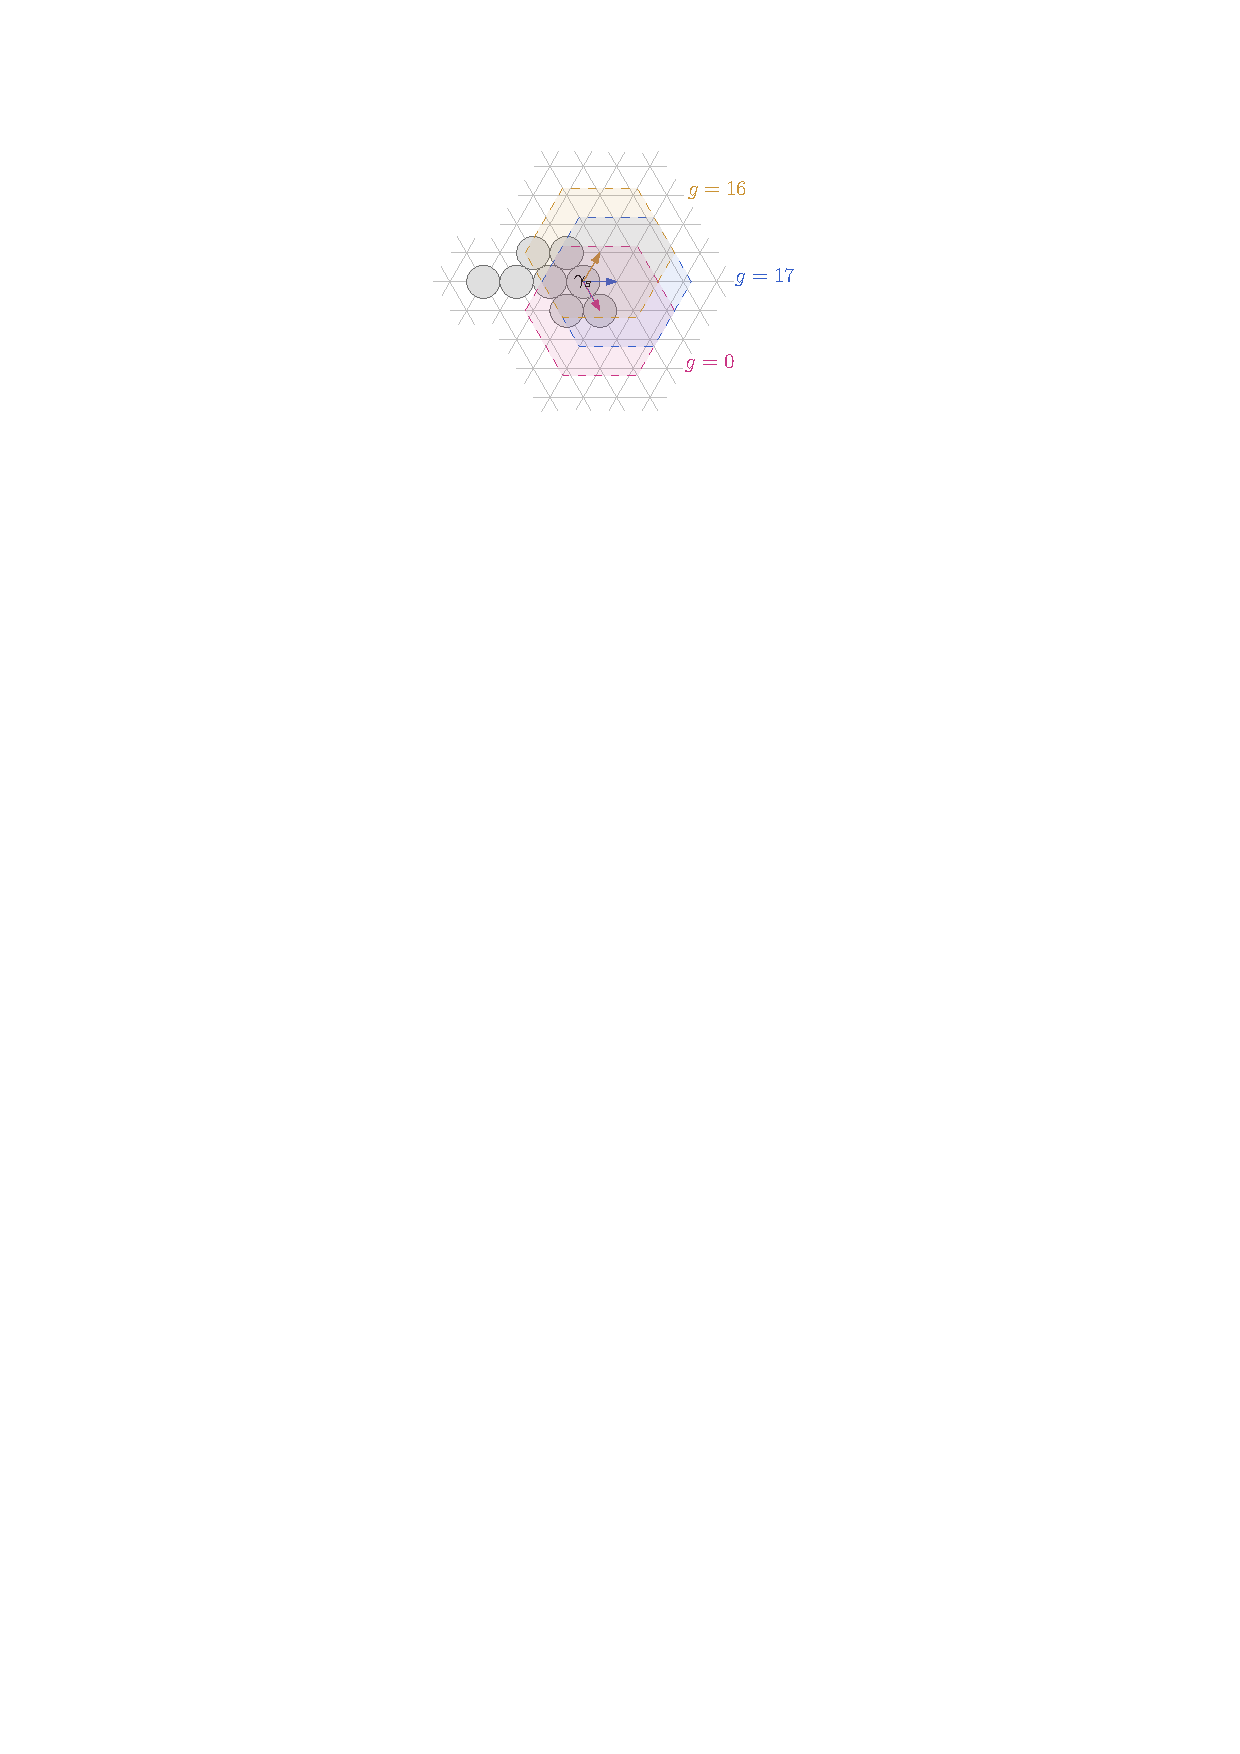
\includegraphics{graphics/ch5_principaldirection.pdf}
    \caption[Principal direction]{The principal direction is chosen from one of three x-monotone options, here illustrated in different colors. The arrows represent the direction $\alpha$. The colored circles cover the two-step neighborhood $\Gamma^2(\coord_s + \alpha)$. From the previously assigned coordinates in $d_i$---the grey disks---within that area follows $g = g(\alpha)$.}
    \label{fig:ch5-principaldirection}
\end{figure}

The principal direction is determined by the free space around $\coord_s + \alpha$, weighed by distance according to a weighting function $g(i, \alpha)$. Refer to Figure~\ref{fig:ch5-principaldirection} together with the following definition of $g$:

\begin{equation*}
g(i, \alpha) = \begin{cases}
    1 & \text{ if } i=0 \text{ and } \alpha = \overrightarrow e(0^\circ), \\
    f(i, \Gamma^2(\coord_s + \alpha)) + f(i, \Gamma(\coord_s + \alpha)) & \text{ if } i>0 \text{ and } f(i, \coord_s + \alpha) = 1, \\
    0 & \text{ otherwise.}
\end{cases}
\end{equation*}

The weight function $g$ evaluates a direction $\alpha$ as ``no space'' if it is not possible to embed the next spine vertex in direction $\alpha$ because the coordinates are immediately blocked.
Among the free two-step neighbors, it gives more weight to the immediately adjacent free coordinates by counting them twice (recall that $\Gamma(\coord) \subset \Gamma^2(\coord)$). These coordinates are available for both branch and leaf disks, rather than those suitable only for leaves.

At the first step only, when there is no maximum embedded spine vertex $v_j$, the principal direction is fixed to ``straight right'' without loss of generality.
The principal direction is evaluated only when embedding a spine vertex. The same principal direction then applies for embedding all adjacent branches and their leaves. Therefore, the direction which maximises the free space at index $i$ is the principal direction, i.e. 

\begin{equation*}
\alpha = \begin{cases}\underset{\alpha}{\arg \max}\, g(i, \alpha) & \text{ if $v_i \in \Spines$}\\
\underset{\alpha}{\arg \max}\, g(j-1, \alpha) & \text{ otherwise}
\end{cases}
\end{equation*}

Let $\coord^- = (x^-, y^-) = d_i(p(v_{i+1}))$ be the assigned x- and y-coordinate of the parent of the next vertex in order $\order$, and let $\alpha = \overrightarrow e(\beta)$ be the principal direction.

\begin{figure}
    \centering
    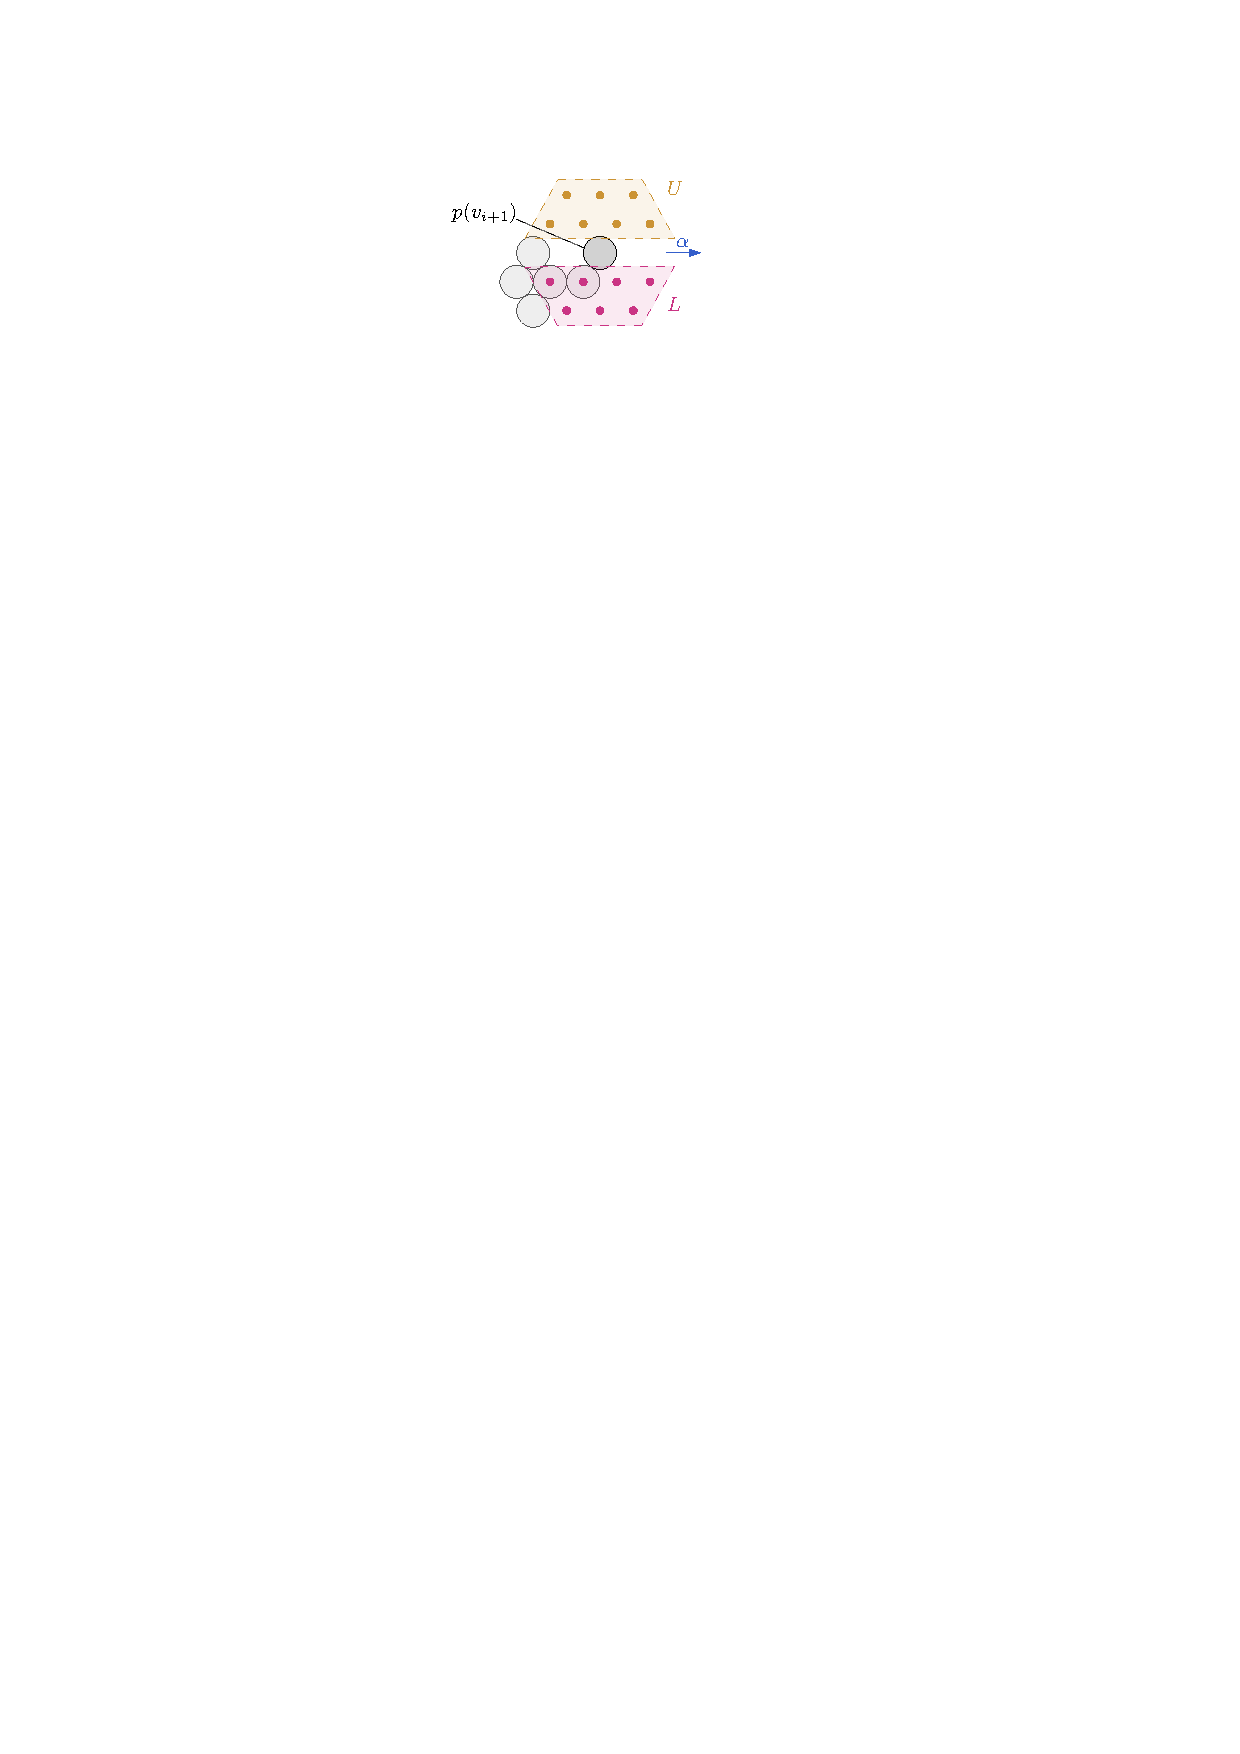
\includegraphics{graphics/ch5_affinity.pdf}
    \caption[Affinity]{The affinity biases the heuristic towards the upper or lower area, whichever contains more (weighted) free space. In this example, the coordinates marked by dots are part of the colored upper and lower area, which are determined from the position of the parent vertex disk in emphasized black and the principal direction $\alpha$.}
    \label{fig:ch5-affinity}
\end{figure}

An x- and y-coordinate $\coord = (x^- + x, y^- + y)$ are \emph{upper coordinates} if $x \cdot \sin (-\beta) + y \cdot \cos (-\beta) > 0$. They are \emph{lower coordinates} if $x \cdot \sin (-\beta) + y \cdot \cos (-\beta) < 0$. Refer to  Figure~\ref{fig:ch5-affinity} for a visualization.
The set $U = \{ \coord \in \Gamma^2(\coord^-) \mid \coord \text{ are upper coordinates} \}$ is the \emph{upper area} and $L = \{ \coord \in \Gamma^2(\coord^-) \mid \coord \text{ are lower coordinates} \}$ is the \emph{lower area}.
The \emph{affinity} $a \in \{-1, 1\}$ at step $i$ of the algorithm guides its decision for embedding of branches and leaves. It is defined as

\begin{equation*}
a = \begin{cases}1 & \text{ if } i = 0 \text{ or } f(i, L) \leq f(i, U), \\
-1 & \text{ otherwise.}
\end{cases}
\end{equation*}

Affinity compares available space ``above'' and ``below'' a line imagined through the parent coordinates $\coord^-$ along the principal direction. The heuristic thereby gains a tendency to embed a branch on the more spacious side of the spine, overall balancing disks on both sides. Coordinates on the side indicated by $a$ are preferred for assignment as described later in this chapter.
Although our definition includes the special case of $i=0$, in which there is no parent vertex, this default has no bearing in practice because decisions on spine vertices are not affected by affinity.

We are now ready to formulate the criteria which apply in the selection of the $\texttt{heuristic}$ function output to determine our heuristic strategy.

\begin{enumerate}
    \item \emph{Bend heuristic}: When deciding the embedding coordinates for a spine vertex, we take a step in the principal direction from the previous spine vertex coordinates. This implements design goal~\ref{dg_bend}.
    \item \emph{Packing heuristic}: For branches and leaves, we prefer coordinates which lie further in the opposite of the principal direction. This implements design goal~\ref{dg_back}.
    \item \emph{Balance heuristic}: For branches and leaves, we strictly prefer coordinates matching the affinity. This implements design goal~\ref{dg_balance}.
    \item \emph{Space criterion}: Coordinates with too few free neighboring coordinates to fit all the leaves are not valid branch candidates. This implements design goal~\ref{dg_space}.
\end{enumerate}

Among these decision criteria, higher precedence is given akin to lexicographical order. For branches and leaves in particular, the space criterion trumps balance, which trumps packing.

\begin{algorithm}[p]
\SetKwFunction{Heuristic}{heuristic}
\SetKwFunction{PrincipalDirection}{principal\_direction}
\SetKwFunction{Affinity}{affinity}
\SetKw{Fail}{fail}
\SetKwData{G}{G}
\SetKwData{undef}{undef}
\SetKwData{Fundament}{F}
\SetKwProg{Fn}{Function}{}{}

\Fn{\Heuristic{$v_{i+1}, d_i$}}{
\KwIn{next vertex $v_{i+1}$, partial embedding function $d_i$}
\KwOut{embedding coordinates for $v_{i+1}$}
\KwData{lobster $G = (\Spines \dotcup \Branches \dotcup \Leaves, E)$, candidate coordinates $\kappa$}
$\coord_s \gets \max(v \in \Spines \wedge v \order v_{i+1})$\;
$\alpha \gets \PrincipalDirection(d_i, \coord_s)$\tcp*{bend heuristic}
\If{$v_{i+1} \in \Spines$}{
    \Return{$\coord_s + \alpha$}\;
}
$\coord_p \gets p(v_{i+1})$\;
$a \gets \Affinity(d_i, \coord_p, \alpha)$\tcp*{balance heuristic}
\For(\tcp*[f]{packing heuristic}){$\beta \text{ in } 180^\circ, 120^\circ, 60^\circ, 0^\circ, -60^\circ, -120^\circ$}{
    $\kappa \gets \coord_p + R(a \cdot \beta) \cdot \alpha$\;
    \If{$f(i, \kappa)$}{
        $\mathcal L \gets \{ l \in \Leaves \mid (v_i, l) \in E \}$\;
        \If(\tcp*[f]{space criterion}){$f(i, \Gamma(\kappa)) \geq |\mathcal L|$}{
            \Return{$\kappa$}\;
        }
    }
}
\Fail{}\tcp*{no representation found}

}
\caption[Heuristic decision function]{The heuristic decision function. We use the embedding order $\order$, the parent function $p$, the neighborhood function $\Gamma$ and the free space function $f$. The rotation matrix $R(\theta) = \begin{bmatrix}\cos \theta & -\sin \theta \\ \sin \theta & \cos \theta \end{bmatrix}$ helps us orient candidates relative to the principal direction $\alpha$.}
\label{alg:heuristic}
\end{algorithm}

The pseudocode in Algorithm~\ref{alg:heuristic} describes how the elements of the heuristic function come together. The spine bends in the principal direction, which promises the most free space. We evaluate candidate coordinates in back-to-front order to encourage tight packing. We distribute branches evenly above and below the spine by affinity, which tends to preserve the x-monotone spine coordinates as unassigned. We embed branches only where there is enough space left for leaves.

Consider this example involving precedence of the different considerations. If the next vertex is a branch and there are ``far-back'' candidate coordinates at $\coord_s + \overrightarrow e(-120^\circ)$, when the affinity is $a=1$, the upper area candidate at $\coord_s + \overrightarrow e(60^\circ)$ is preferred. If there are 4 leaves on the branch and not enough free space in the neighborhood of the preferred candidate, $\coord_s + \overrightarrow e(0^\circ)$ is chosen instead, and so on until some candidate satisfies the space criterion.

\section{Breadth-First Order}
\label{section:ch5-bfs}

We also examine a variant of the heuristic algorithm that uses a different vertex embed order, denoted $\order^B$.
The original definition for $\order^D$ permits the case that, while embedding a particular subtree (branch and leaves), the algorithm might embed a leaf at critical coordinates that would have been required as a free space for embedding some later branch vertex. Instead of embedding all the leaves on a branch directly after the branch vertex, the variant definition orders all branch vertices with the same parent spine to be embedded directly following that spine. Only then does it consider all the adjacent leaves.

We call this variant order the \emph{breadth-first} order to distinguish it from the previously defined depth-first order.
A breadth-first embedding order $\order^B$ is \emph{admissible} if it fulfills the following criteria, analogous to admissibility for a depth-first order.

\begin{itemize}
    \item $\order^B$ is a total order. It is reflexive, transitive and antisymmetric.
    \item $\order^B$ orders the spine like an admissible depth-first order.
    \item $\order^B$ groups branches and leaves together with their parent spine. 
     Let $s_1, s_2 \in \Spines, b \in \Branches, l \in \Leaves$ and $s_1 \order^B s_2$. If $s_1 = p(b)$, then $b \order^B s_2$. If $s_1 = p(p(l))$, then $l \order^B s_2$.
    \item $\order^B$ groups branches before leaves in a subtree. Let $s \in \Spines, b \in \Branches, l \in \Leaves, s = p(b)$ and $s = p(p(l))$. Then $b \order^B l$.
    \item Parent vertices come first. Let $v_1, v_2 \in V$. If $v_1 = p(v_2)$, then $v_1 \order^B v_2$.
\end{itemize}

Otherwise, the definition of the algorithm and heuristic function remain the same.
